% This is the default LaTeX template (default-1.17.0.2.tex) from the RMarkdown package, from:
% https://github.com/rstudio/rmarkdown/blob/master/inst/rmd/latex/default-1.17.0.2.tex
%
% New additions to the template are marked with "LCR"

%\documentclass[$if(fontsize)$$fontsize$,$endif$$if(lang)$$babel-lang$,$endif$$if(papersize)$$papersize$paper,$endif$$for(classoption)$$classoption$$sep$,$endfor$]{$documentclass$} %LCR
$if(book_size)$ % if the book is being rendered for print, force twoside option
\documentclass[$if(fontsize)$$fontsize$,$endif$$if(papersize)$$papersize$paper,twoside,$endif$$for(classoption)$$classoption$$sep$,$endfor$]{$documentclass$} %LCR
% \documentclass[twoside,openright]{book}
$else$ % if not, force the oneside and a4paper options, which seem to be the only reasonable defaults
\documentclass[$if(fontsize)$$fontsize$,$endif$a4paper,oneside,$for(classoption)$$classoption$$sep$,$endfor$]{$documentclass$} %LCR
$endif$
$if(fontfamily)$
\usepackage[$for(fontfamilyoptions)$$fontfamilyoptions$$sep$,$endfor$]{$fontfamily$}
$else$
\usepackage{lmodern}
$endif$
$if(linestretch)$
\usepackage{setspace}
\setstretch{$linestretch$}
$endif$
\usepackage{amssymb,amsmath}
\usepackage{ifxetex,ifluatex}
\usepackage{fixltx2e} % provides \textsubscript
\ifnum 0\ifxetex 1\fi\ifluatex 1\fi=0 % if pdftex
  \usepackage[$if(fontenc)$$fontenc$$else$T1$endif$]{fontenc}
  \usepackage[utf8]{inputenc}
$if(euro)$
  \usepackage{eurosym}
$endif$
\else % if luatex or xelatex
  \ifxetex
    \usepackage{mathspec}
  \else
    \usepackage{fontspec}
  \fi
  \defaultfontfeatures{Ligatures=TeX,Scale=MatchLowercase}
$if(euro)$
  \newcommand{\euro}{€}
$endif$
$if(mainfont)$
    \setmainfont[$for(mainfontoptions)$$mainfontoptions$$sep$,$endfor$]{$mainfont$}
$endif$
$if(sansfont)$
    \setsansfont[$for(sansfontoptions)$$sansfontoptions$$sep$,$endfor$]{$sansfont$}
$endif$
$if(monofont)$
    \setmonofont[Mapping=tex-ansi$if(monofontoptions)$,$for(monofontoptions)$$monofontoptions$$sep$,$endfor$$endif$]{$monofont$}
$endif$
$if(mathfont)$
    \setmathfont(Digits,Latin,Greek)[$for(mathfontoptions)$$mathfontoptions$$sep$,$endfor$]{$mathfont$}
$endif$
$if(CJKmainfont)$
    \usepackage{xeCJK}
    \setCJKmainfont[$for(CJKoptions)$$CJKoptions$$sep$,$endfor$]{$CJKmainfont$}
$endif$
\fi
% use upquote if available, for straight quotes in verbatim environments
\IfFileExists{upquote.sty}{\usepackage{upquote}}{}
% use microtype if available
\IfFileExists{microtype.sty}{%
\usepackage{microtype}
\UseMicrotypeSet[protrusion]{basicmath} % disable protrusion for tt fonts
}{}
$if(book_size)$ % LCR
\usepackage[paperwidth=170mm,paperheight=240mm, includeheadfoot, asymmetric]{geometry} % LCR %set to standard thesis size
\geometry{$for(geometry)$$geometry$$sep$,$endfor$}
$endif$
% $if(geometry)$
% $if(book_size)$ % LCR % if we've already invoked geometry
% \geometry{$for(geometry)$$geometry$$sep$,$endfor$} %LCR % don't call usepackage again
% $else$ %LCR
% \usepackage[$for(geometry)$$geometry$$sep$,$endfor$]{geometry}
% $endif$
% $endif$ %LCR
\usepackage{hyperref}
$if(colorlinks)$
\PassOptionsToPackage{usenames,dvipsnames}{color} % color is loaded by hyperref
$endif$
\hypersetup{unicode=true,
$if(title-meta)$
            pdftitle={$title-meta$},
$endif$
$if(author-meta)$
            pdfauthor={$author-meta$},
$endif$
$if(keywords)$
            pdfkeywords={$for(keywords)$$keywords$$sep$; $endfor$},
$endif$
$if(colorlinks)$
            colorlinks=true,
            linkcolor=$if(linkcolor)$$linkcolor$$else$Maroon$endif$,
            citecolor=$if(citecolor)$$citecolor$$else$Blue$endif$,
            urlcolor=$if(urlcolor)$$urlcolor$$else$Blue$endif$,
$else$
            pdfborder={0 0 0},
$endif$
            breaklinks=true}
\urlstyle{same}  % don't use monospace font for urls
$if(lang)$
\ifLuaTeX
\usepackage[bidi=basic]{babel}
\else
\usepackage[bidi=default]{babel}
\fi
$if(babel-lang)$
\babelprovide[main,import]{$babel-lang$}
$if(mainfont)$
\ifPDFTeX
\else
\babelfont{rm}[$for(mainfontoptions)$$mainfontoptions$$sep$,$endfor$$if(mainfontfallback)$,RawFeature={fallback=mainfontfallback}$endif$]{$mainfont$}
\fi
$endif$
$endif$
$for(babel-otherlangs)$
\babelprovide[import]{$babel-otherlangs$}
$endfor$
$for(babelfonts/pairs)$
\babelfont[$babelfonts.key$]{rm}{$babelfonts.value$}
$endfor$
% get rid of language-specific shorthands (see #6817):
\let\LanguageShortHands\languageshorthands
\def\languageshorthands#1{}
$endif$
$for(header-includes)$
$header-includes$
$endfor$
$if(natbib)$
\usepackage$if(natbiboptions)$[$for(natbiboptions)$$natbiboptions$$sep$,$endfor$]$endif${natbib}
\bibliographystyle{$if(biblio-style)$$biblio-style$$else$plainnat$endif$}
$endif$
$if(biblatex)$
\usepackage$if(biblio-style)$[style=$biblio-style$]$endif${biblatex}
$if(biblatexoptions)$\ExecuteBibliographyOptions{$for(biblatexoptions)$$biblatexoptions$$sep$,$endfor$}$endif$
$for(bibliography)$
\addbibresource{$bibliography$}
$endfor$
$endif$
$if(listings)$
\usepackage{listings}
\newcommand{\passthrough}[1]{#1}
$endif$
$if(lhs)$
\lstnewenvironment{code}{\lstset{language=Haskell,basicstyle=\small\ttfamily}}{}
$endif$
$if(highlighting-macros)$
$highlighting-macros$
$endif$
$if(verbatim-in-note)$
\usepackage{fancyvrb}
\VerbatimFootnotes % allows verbatim text in footnotes
$endif$
$if(tables)$
\usepackage{longtable,booktabs}
$endif$
$if(graphics)$
\usepackage{graphicx,grffile}
\makeatletter
\def\maxwidth{\ifdim\Gin@nat@width>\linewidth\linewidth\else\Gin@nat@width\fi}
\def\maxheight{\ifdim\Gin@nat@height>\textheight\textheight\else\Gin@nat@height\fi}
\makeatother
% Scale images if necessary, so that they will not overflow the page
% margins by default, and it is still possible to overwrite the defaults
% using explicit options in \includegraphics[width, height, ...]{}
\setkeys{Gin}{width=\maxwidth,height=\maxheight,keepaspectratio}
$endif$
$if(links-as-notes)$
% Make links footnotes instead of hotlinks:
\renewcommand{\href}[2]{#2\footnote{\url{#1}}}
$endif$
$if(strikeout)$
\usepackage[normalem]{ulem}
% avoid problems with \sout in headers with hyperref:
\pdfstringdefDisableCommands{\renewcommand{\sout}{}}
$endif$
$if(indent)$
$else$
\IfFileExists{parskip.sty}{%
\usepackage{parskip}
}{% else
\setlength{\parindent}{0pt}
\setlength{\parskip}{6pt plus 2pt minus 1pt}
}
$endif$
\setlength{\emergencystretch}{3em}  % prevent overfull lines
\providecommand{\tightlist}{%
  \setlength{\itemsep}{0pt}\setlength{\parskip}{0pt}}
$if(numbersections)$
\setcounter{secnumdepth}{5}
$else$
\setcounter{secnumdepth}{0}
$endif$
$if(subparagraph)$
$else$
% Redefines (sub)paragraphs to behave more like sections
\ifx\paragraph\undefined\else
\let\oldparagraph\paragraph
\renewcommand{\paragraph}[1]{\oldparagraph{#1}\mbox{}}
\fi
\ifx\subparagraph\undefined\else
\let\oldsubparagraph\subparagraph
\renewcommand{\subparagraph}[1]{\oldsubparagraph{#1}\mbox{}}
\fi
$endif$
$if(dir)$
\ifxetex
  % load bidi as late as possible as it modifies e.g. graphicx
  $if(latex-dir-rtl)$
  \usepackage[RTLdocument]{bidi}
  $else$
  \usepackage{bidi}
  $endif$
\fi
\ifnum 0\ifxetex 1\fi\ifluatex 1\fi=0 % if pdftex
  \TeXXeTstate=1
  \newcommand{\RL}[1]{\beginR #1\endR}
  \newcommand{\LR}[1]{\beginL #1\endL}
  \newenvironment{RTL}{\beginR}{\endR}
  \newenvironment{LTR}{\beginL}{\endL}
\fi
$endif$

% LCR: fix for new required cslreferences environment in pandoc
% from https://github.com/rstudio/rticles/blob/81bb6816a42797f66fbbc6d7c92ffd8216783ed3/inst/rmarkdown/templates/elsevier/resources/template.tex#L146-L177
$if(csl-refs)$
% Pandoc citation processing
\newlength{\cslhangindent}
\setlength{\cslhangindent}{1.5em}
\newlength{\csllabelwidth}
\setlength{\csllabelwidth}{3em}
\newlength{\cslentryspacingunit} % times entry-spacing
\setlength{\cslentryspacingunit}{\parskip}
% for Pandoc 2.8 to 2.10.1
\newenvironment{cslreferences}%
  {$if(csl-hanging-indent)$\setlength{\parindent}{0pt}%
  \everypar{\setlength{\hangindent}{\cslhangindent}}\ignorespaces$endif$}%
  {\par}
% For Pandoc 2.11+
\newenvironment{CSLReferences}[2] % #1 hanging-ident, #2 entry spacing
 {% don't indent paragraphs
  \setlength{\parindent}{0pt}
  % turn on hanging indent if param 1 is 1
  \ifodd #1
  \let\oldpar\par
  \def\par{\hangindent=\cslhangindent\oldpar}
  \fi
  % set entry spacing
  \setlength{\parskip}{#2\cslentryspacingunit}
 }%
 {}
\usepackage{calc}
\newcommand{\CSLBlock}[1]{#1\hfill\break}
\newcommand{\CSLLeftMargin}[1]{\parbox[t]{\csllabelwidth}{#1}}
\newcommand{\CSLRightInline}[1]{\parbox[t]{\linewidth - \csllabelwidth}{#1}\break}
\newcommand{\CSLIndent}[1]{\hspace{\cslhangindent}#1}
$endif$

%%% Use protect on footnotes to avoid problems with footnotes in titles
\let\rmarkdownfootnote\footnote%
\def\footnote{\protect\rmarkdownfootnote}

%%% This fixes a TexLive 2019 change that broke pandoc template. Will also be fixed in pandoc 2.8 %LCR
% https://github.com/jgm/pandoc/issues/5801
\renewcommand{\linethickness}{0.05em}

\usepackage{pdfpages}

%%%%%%%%%%%%% BEGIN DOCUMENT %%%%%%%%%%%%%
\begin{document}

%% Page I: the half-title / "Franse pagina" %LCR
\frontmatter

% Include the book cover as first page


$if(print_version)$
$else$
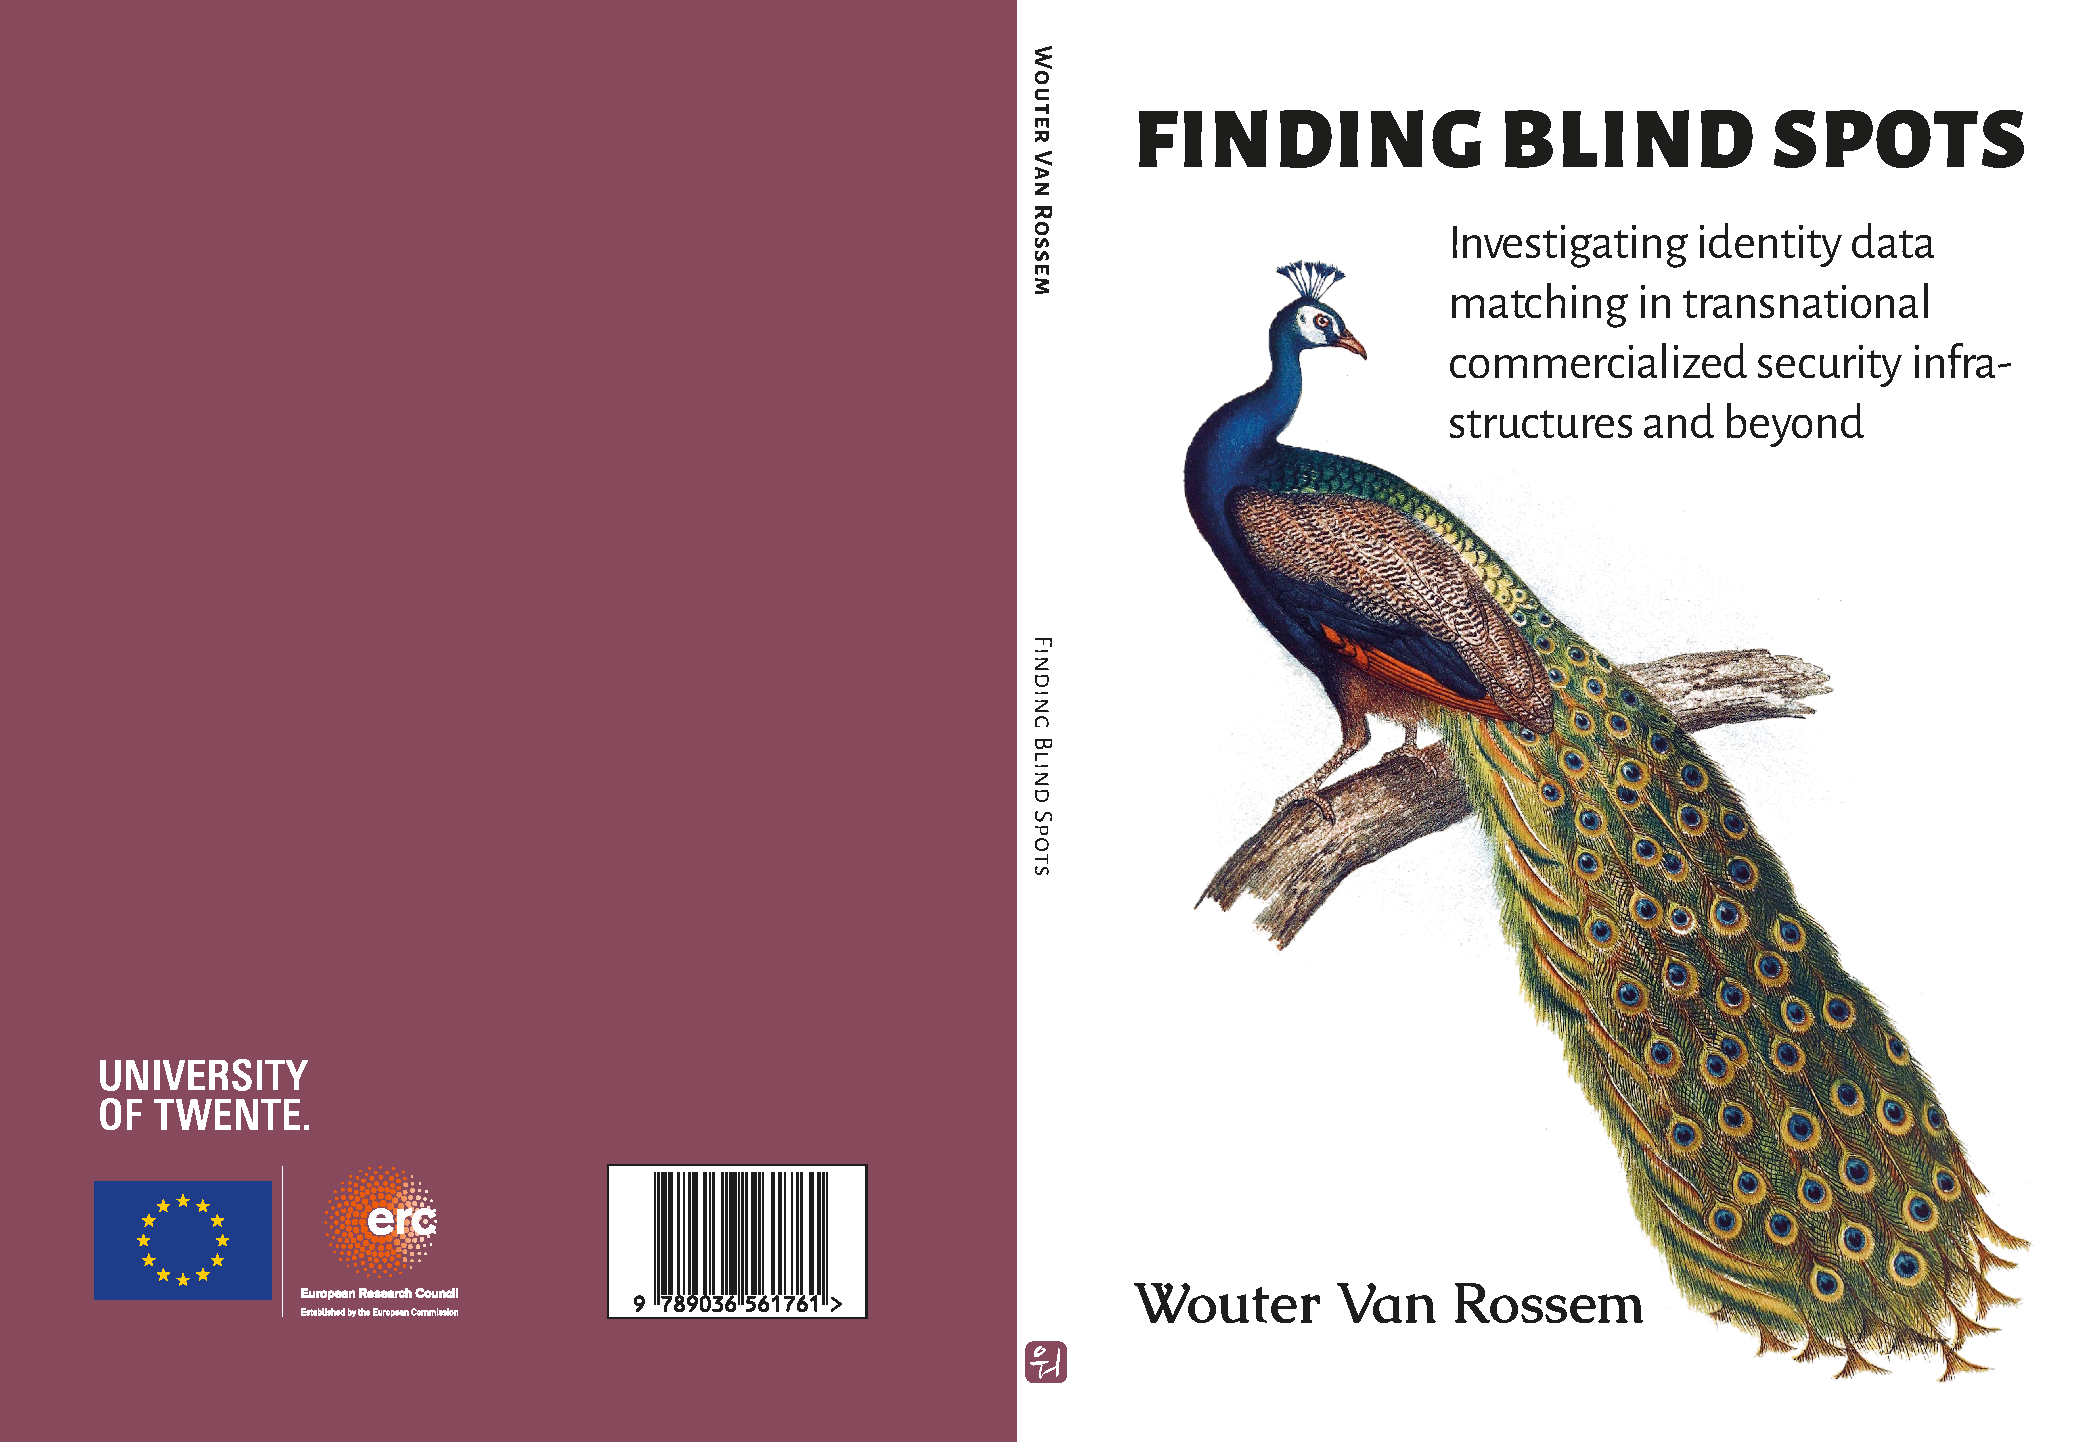
\includepdf[pages=1, fitpaper=true]{book-cover/book-cover-2-sides-compressed.pdf}
$endif$

\thispagestyle{empty}
\def\drop{.1\textheight}

\vspace*{\drop}
\begin{center}
\huge\textbf{\uppercase{$if(title)$$title$$else$[… Title Doctoral Thesis…]$endif$}}\par
$if(subtitle)$
% \vspace{\baselineskip}
\medskip
\Large\uppercase{$subtitle$}\par
$endif$
\vspace{\baselineskip}
{\Large \textit{$if(author)$$author$$else$[…given names in full…] [… surname…]$endif$}}
\end{center}

% \newpage
% \thispagestyle{empty}
% \vspace*{\fill}
% \textit{This page intentionally left blank.}
% \newpage

$if(print_version)$
\clearpage\shipout\null
$endif$

%% Page II: Colophon %LCR
% \clearpage
% \thispagestyle{empty}
% \vspace*{\fill}
% \begingroup % to change formatting only temporarily
% \small
% \setlength{\parskip}{\baselineskip} % add space between paragraphs
% \setlength\parindent{0pt} % no indents
% $if(funder)$
% The investigations in this thesis were supported by $if(grant)$a $grant$ from $endif$
% $if(funder)$$funder$.$endif$
% $endif$

% This thesis was typeset using (R) Markdown, \LaTeX\ and the \verb+bookdown+ R-package. The text is set in Piazolla, a font designed by Juan Pablo del Peral for Huerta Tipográfica.
% $if(ISBN)$\\ ISBN: $ISBN$$endif$$if(printing)$\\ Printing: $printing$$endif$$if(cover)$\\ Cover: $cover$$endif$

% $if(thesis_url)$
% An online version of this thesis is available at $thesis_url$$if(license)$, licensed under a $license$.$endif$
% $endif$
% \endgroup

%% Page III: `Title page' mandated by University of Amsterdam %LCR
\clearpage
\thispagestyle{empty}
\vspace*{\drop}
\begin{center}
\huge\textbf{\uppercase{$if(title)$$title$$else$[… Title Doctoral Thesis…]$endif$}}\par
$if(subtitle)$
% \vspace{\baselineskip}
\medskip
\Large\uppercase{$subtitle$}\par
$endif$
\vfill % this space will be whatever is left on the page
\large \uppercase{dissertation}\par
\vspace{\baselineskip}
\linespread{1.3}{\normalsize to obtain\\
the degree of doctor at the University of Twente,\\
on the authority of the rector magnificus,\\
prof. dr. ir. A. Veldkamp\\ % make sure this is the current rector magnificus
\mbox{on account of the decision of the Doctorate Board,}\\
to be publicly defended\\
on $if(date)$$date$$else$Monday, July 15\textsuperscript{th}, 2024$endif$, at $if(time)$$time$$else$[…time…]$endif$ p.m.}\par %
\vspace*{2cm}
{\normalsize by}\par
\medskip
{\normalsize\textbf{$if(author)$$author$$else$[…given names in full…] [… surname…]$endif$}}\par
\medskip
% {\large born on $if(birthplace)$$birthplace$$else$[…place of birth…]$endif$}
\normalsize born on the 7\textsuperscript{th} of August, 1989\\
in Brussels, Belgium
\end{center}

$if(print_version)$
\clearpage\shipout\null
$endif$

%% Page IV: info on thesis committee %LCR
\clearpage
\thispagestyle{empty}
\noindent\text{This dissertation has been approved by:}\\
\\
\noindent\begin{tabular}{@{}lll}

$if(one_promotor)$Promotor:$else$Promotores:$endif$
$for(promotores)$
& $if(promotores.title)$ $promotores.title$$else$ […full title…]$endif$$if(promotores.initials)$ $promotores.initials$$else$ […initials…]$endif$$if(promotores.surname)$ $promotores.surname$$else$ […surname…]$endif$\\
$endfor$

$if(copromotores)$
$if(one_copromotor)$Co-promotor:$else$Co-promotors:$endif$
$for(copromotores)$
& $if(copromotores.title)$ $copromotores.title$$else$ […full title…]$endif$$if(copromotores.initials)$ $copromotores.initials$$else$ […initials…]$endif$$if(copromotores.surname)$ $copromotores.surname$$else$ […surname…]$endif$\\
$endfor$
$endif$
\end{tabular}\\

\vspace*{\fill}
\begingroup % to change formatting only temporarily
\small
\setlength{\parskip}{\baselineskip} % add space between paragraphs
\setlength\parindent{0pt} % no indents
% $if(funder)$
% The investigations in this dissertation were supported by $if(grant)$a $grant$ from $endif$
The investigations in this dissertation were conducted within the context of the “Processing Citizenship: Digital registration of migrants as co-production of citizens, territory and Europe” project, which has received funding from the European Research Council under the European Union’s Horizon 2020 research and innovation programme under grant agreement No 714463.
% $if(funder)$$funder$.$endif$
% $endif$

\vspace{\baselineskip}

This dissertation was typeset using (R) Markdown, \LaTeX\ and the \verb+bookdown+ R-package. The text is set in Alegreya, a font designed by Juan Pablo del Peral for Huerta Tipográfica.

\vspace{\baselineskip}

The cover design was created by Wouter Van Rossem, featuring Figure 224 “Der gemeine Pfau (Pave cristatus)” from Fitzinger’s “Bilder-atlas zur Wissenschaftlich-populären Naturgeschichte der Vögel in ihren sämmtlichen Hauptformen” (1864), sourced from \url{https://www.biodiversitylibrary.org/page/33050550}."
\vspace{\baselineskip}
% $if(cover)$\\ Cover design: $cover$$endif$

$if(printing)$Printed by: $printing$$endif$$if(layout)$\\ Lay-out: $printing$$endif$$if(ISBN1)$ ISBN (print): $ISBN1$$endif$$if(ISBN2)$\\ ISBN (digital): $ISBN2$$endif$$if(DOI)$\\ DOI: $DOI$$endif$$if(thesis_url)$\\ URL: $thesis_url$$endif$

% $if(thesis_url)$
% An online version of this thesis is available at $thesis_url$$if(license)$, licensed under a $license$.$endif$
% $endif$

\vspace{\baselineskip}

© 2024 $if(author)$$author$$else$[…given names in full…] [… surname…]$endif$, Enschede, The Netherlands and Bologna, Italy. This work is licensed under the Creative Commons Attribution-NonCommercial-ShareAlike 4.0 International License. To view a copy of this license, visit \url{http://creativecommons.org/licenses/by-nc-sa/4.0/}. No parts of this dissertation may be reproduced, stored in a retrieval system or transmitted in any form or by any means for commercial purposes without permission of the author. If you remix, transform, or build upon the material, you must distribute your contributions under the same license as the original.
\endgroup

$if(print_version)$
\clearpage\shipout\null
$endif$

%%%%%%%%%%%%%%%%%%

\clearpage
\thispagestyle{empty}
\noindent

\textbf{Graduation Committee}\\

% \begin{tabular}{@{}ll}
\begin{tabular}{p{0.3\linewidth}p{0.6\linewidth}}
Chair / Secretary: & prof. dr. T. Bondarouk \\
& \\
Promotor: & prof. dr. S. Kuhlmann \\
          & \textit{University of Twente, BMS, Knowledge, Transformation \& Society} \\
& \\
Co-promotors: & prof. dr. A. Pelizza \\
              & \textit{University of Bologna, Department of Philosophy, and Aarhus University, Department of Digital Design and Information Studies} \\
& \\
              & prof. dr. ir. M. van Keulen \\
              & \textit{University of Twente, EEMCS, Datamanagement \& Biometrics} \\
& \\
Committee Members: $for(members)$
& $if(members.title)$ $members.title$$else$ […full title…]$endif$$if(members.initials)$ $members.initials$$else$ […initials…]$endif$$if(members.surname)$ $members.surname$$else$ […surname…]$endif$ \\
& \textit{$if(members.affiliation)$$members.affiliation$$else$ & […affiliation…]$endif$}\\
& \\
$endfor$

\end{tabular}

% \text{} & Universiteit Twente, BMS, Knowledge, Transformation & Society\\

% \noindent Faculteit: $if(faculty)$$faculty$$else$[…name faculty…]$endif$

$if(print_version)$
\clearpage\shipout\null
$endif$

% Dedication page
\newpage
\thispagestyle{empty}
\vspace*{\fill}
\begin{center}
    \textit{In memory of my mother, Linda Liekendael (1960–2020)}
\end{center}
\vspace*{\fill}

%%%%%%%%%%%%%%%%%%

$if(abstract)$
\begin{abstract}
$abstract$
\end{abstract}
$endif$

$for(include-before)$
$include-before$

$endfor$
$if(toc)$
{
$if(colorlinks)$
\hypersetup{linkcolor=$if(toccolor)$$toccolor$$else$black$endif$}
$endif$
\setcounter{tocdepth}{$toc-depth$}
\tableofcontents
}
$endif$
$if(lot)$
\listoftables
$endif$
$if(lof)$
\listoffigures
$endif$
\mainmatter
$body$

\backmatter
$if(natbib)$
$if(bibliography)$
$if(biblio-title)$
$if(book-class)$
\renewcommand\bibname{$biblio-title$}
$else$
\renewcommand\refname{$biblio-title$}
$endif$
$endif$
\bibliography{$for(bibliography)$$bibliography$$sep$,$endfor$}

$endif$
$endif$
$if(biblatex)$
\printbibliography$if(biblio-title)$[title=$biblio-title$]$endif$

$endif$
$for(include-after)$
$include-after$

$endfor$

\end{document}